\documentclass[aspectratio=169,11pt]{beamer}
\usepackage{fathomnet-course}
\title{\coursetitle}
\subtitle{\coursesubtitle\\[2pt]\small Session 1 -- Kick-off and roadmap}
\date{}
\author{}
\begin{document}
\maketitle

% ---------------------------------------------------------------------------
\begin{frame}{The problem: too many videos, too few taxonomists}
\begin{columns}[T]
\column{0.55\textwidth}
\begin{itemize}
  \item Remotely operated vehicles (ROVs) film the deep sea for \hl{thousands of hours} per year.
  \item Every animal in every frame should be \emph{identified} and \emph{counted}: biodiversity surveys, monitoring of mining areas, climate change.
  \item Annotation is done by \hl{experts by hand} -- the bottleneck of deep-sea ecology.
  \item Idea: let a computer propose the identification, the expert checks it.
\end{itemize}
\column{0.42\textwidth}
\begin{block}{The question of this project}
\large Can a computer learn to identify deep-sea animals -- and \hl{when can we trust it}?
\end{block}
\end{columns}
\end{frame}

\begin{frame}{FathomNet and the FathomNet 2025 challenge}
\begin{itemize}
  \item \textbf{FathomNet} (MBARI and partners): an open database of underwater images in which experts have drawn a \emph{box} around each animal and named it.
  \item \textbf{FathomNet 2025} (Kaggle, CVPR 2025 workshop): build a program that names the animal in each box.
  \item Scored \emph{biologically}: confusing two rockfish species is a small mistake; confusing a sea star with a jellyfish is a big one (distance in the tree of life, 0--12).
\end{itemize}
\vspace{4pt}
\begin{exampleblock}{What we use}
The official training set: \textbf{8,981 images}, \textbf{23,699 boxes}, \textbf{79 labels}, about 300 boxes per label.\\
We cut every box out as a small $224\times224$ picture (a \emph{crop}): \textbf{23,698 crops}, 250\,MB.
\end{exampleblock}
\end{frame}

\begin{frame}{Meet the animals}
\centering
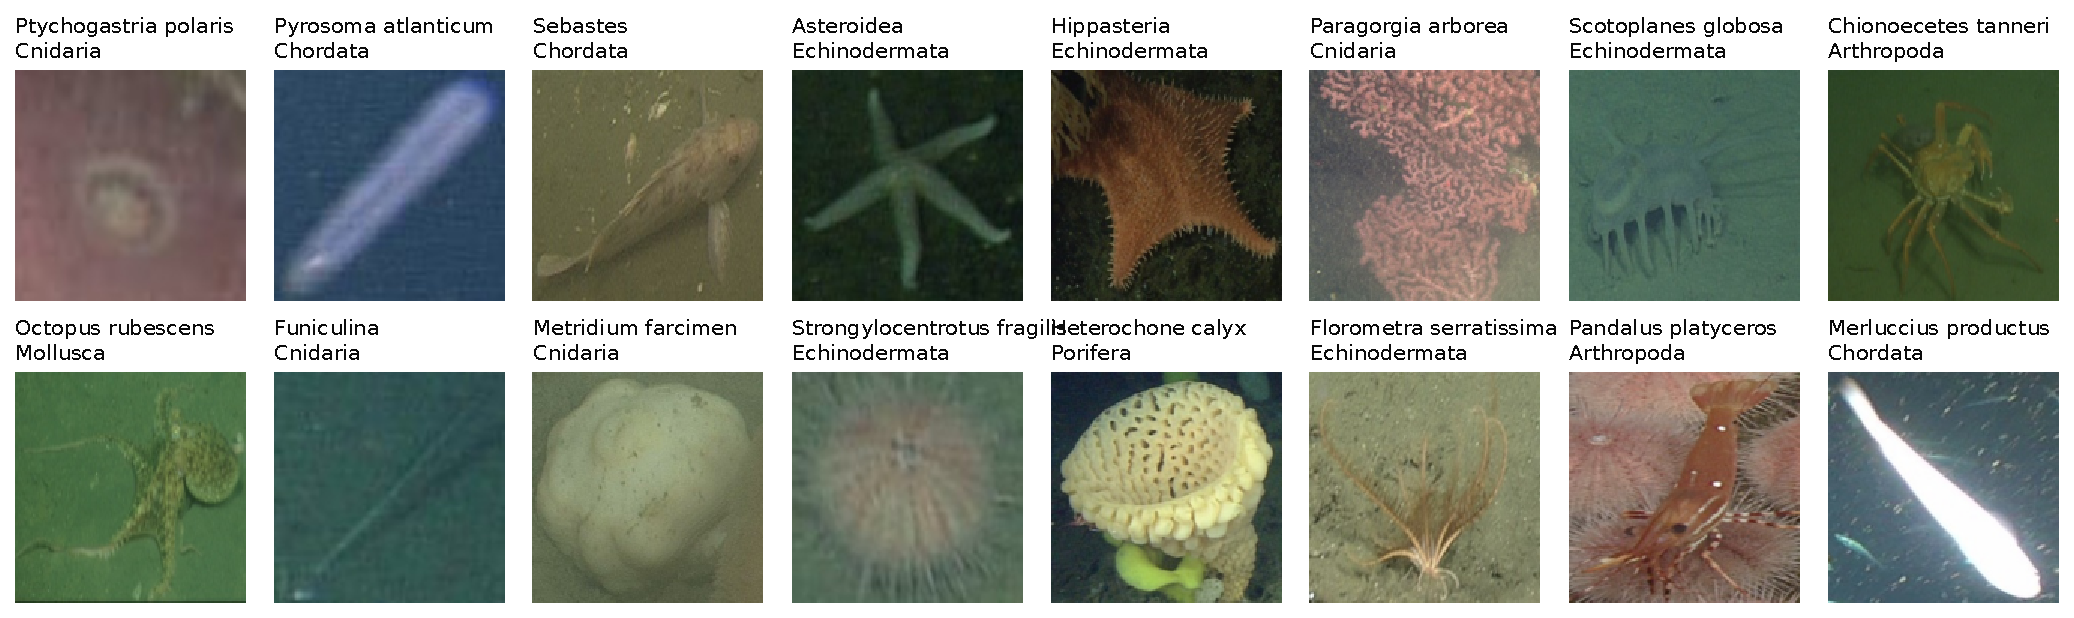
\includegraphics[width=\linewidth]{figures/animals_grid.pdf}\\[4pt]
\small 16 of the 79 labels -- one crop each, with its phylum. Crops are $224\times224$ pixels; many are much blurrier than these.
\end{frame}

\begin{frame}{79 labels, 7 phyla -- and labels at different ranks}
\begin{columns}[c]
\column{0.52\textwidth}
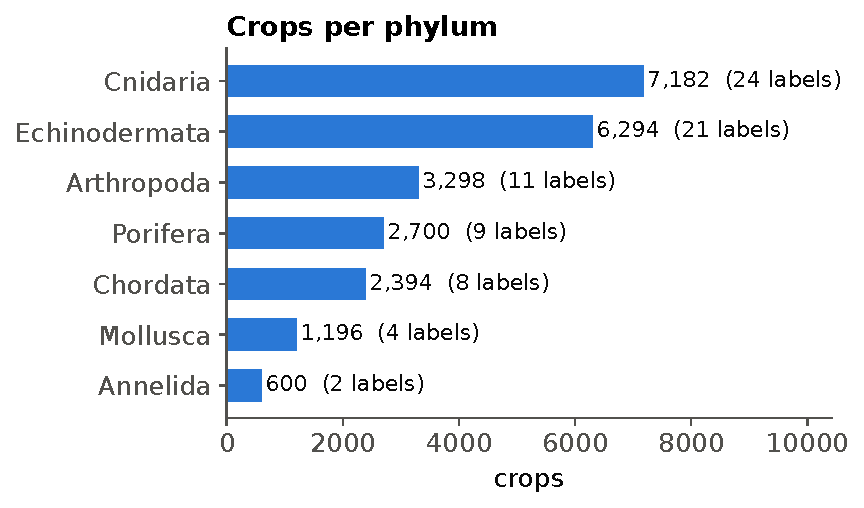
\includegraphics[width=\linewidth]{figures/phylum_counts.pdf}
\column{0.45\textwidth}
\small
\begin{tabular}{@{}lr@{}}
\toprule
label is a \dots & labels \\
\midrule
species (\emph{Sebastes diploproa}) & 33 \\
genus (\emph{Sebastes}) & 21 \\
family (Elpidiidae) & 8 \\
order (Actiniaria) & 6 \\
class (Asteroidea) & 6 \\
phylum (Porifera) & 1 \\
other rank (Tunicata, \dots) & 4 \\
\bottomrule
\end{tabular}

\vspace{6pt}
\muted{Experts only name what they can see. A blurry sea star stays ``Asteroidea''.}
\end{columns}
\end{frame}

% ---------------------------------------------------------------------------
\section{What is a classifier?}

\begin{frame}{A classifier is an identification key that is learned from examples}
\centering
\begin{tikzpicture}[node distance=7mm, box/.style={draw=ocean, rounded corners, fill=sea!8, minimum height=13mm, align=center, text width=27mm}, >=Stealth]
  \node[box] (img) {\textbf{animal}\\\small(a crop)};
  \node[box, right=of img] (feat) {\textbf{characters}\\\small numbers: colour, shape, \dots};
  \node[box, right=of feat] (rule) {\textbf{rule}\\\small learned from labelled examples};
  \node[box, right=of rule, fill=coral!15, draw=coral] (lab) {\textbf{label}\\\small ``Asteroidea''};
  \draw[->, thick] (img) -- (feat);
  \draw[->, thick] (feat) -- (rule);
  \draw[->, thick] (rule) -- (lab);
  \node[below=4mm of feat, text=muted, font=\small] {``features''};
  \node[below=4mm of rule, text=muted, font=\small] {``model''};
\end{tikzpicture}

\vspace{10pt}
\begin{tabularx}{0.9\linewidth}{@{}XX@{}}
\toprule
\textbf{Biology} & \textbf{Machine learning} \\
\midrule
reference collection & training set \\
character (colour, number of arms) & feature \\
species / taxon name & class, label \\
identification key, field guide & classifier, model \\
blind test with new specimens & test set \\
\bottomrule
\end{tabularx}
\end{frame}

\begin{frame}{What you will be able to do at the end}
\begin{enumerate}
  \item \textbf{Explain} what a classifier is, what ``training'' and ``testing'' mean, and why we must never test on the training examples.
  \item \textbf{Describe} an image with numbers (\emph{features}) -- from raw pixels over hand-made characters to what a neural network ``sees''.
  \item \textbf{Use} six different classifiers (nearest centroid, $k$-nearest neighbours, decision tree, random forest, logistic regression, neural network) and compare them fairly.
  \item \textbf{Read} the results: accuracy, confusion matrix, per-label scores -- and judge mistakes \emph{biologically}.
  \item \textbf{Judge} when a classifier can be trusted for a real survey.
\end{enumerate}
\vspace{4pt}
\muted{You need no programming experience beyond changing a few words in a notebook. No GPU needed.}
\end{frame}

% ---------------------------------------------------------------------------
\section{The roadmap}

\begin{frame}{Roadmap: six sessions}
\centering
\begin{tikzpicture}[x=2.45cm, >=Stealth,
  wk/.style={circle, fill=ocean, text=white, font=\bfseries\small, minimum size=8mm, inner sep=0},
  lab/.style={text width=21mm, align=center, font=\scriptsize, anchor=north},
  ttl/.style={text width=22mm, align=center, font=\footnotesize\bfseries, text=ocean, anchor=south}]
  \draw[line width=2.2pt, sea!40] (0.7,0) -- (6.3,0);
  \foreach \i/\t/\l in {
    1/Kick-off\\ \& the data/{Lab 0: set up, download, look at the animals},
    2/What is a\\ classifier?/{Lab 1: your first classifier, by hand and by computer},
    3/How a computer\\ sees an animal/{Lab 2: pixels, characters, CNN features; the classifier zoo},
    4/Testing\\ honestly/{Lab 3: confusion matrix, tree-of-life mistakes, new dives},
    5/Mini-\\challenge/{Lab 4: beat the class leaderboard; poster},
    6/Final\\ exam/{90 min written exam; poster session}} {
    \node[wk] (w\i) at (\i,0) {\i};
    \node[ttl] at (\i,0.55) {\t};
    \node[lab] at (\i,-0.5) {\l};
  }
  \node[wk, fill=coral] at (6,0) {6};
\end{tikzpicture}
\end{frame}

\begin{frame}{Week by week}
\small
\begin{tabularx}{\linewidth}{@{}c>{\raggedright}p{3.1cm}>{\raggedright\arraybackslash\ttfamily\scriptsize}p{4.0cm}X@{}}
\toprule
& \textbf{Session (slides)} & \textbf{Lab notebook} & \textbf{You hand in} \\
\midrule
1 & Kick-off \& roadmap & lab0\_data & dataset loads; one figure of ``your'' animal group \\
2 & What is a classifier? & lab1\_first\_classifier & answers to the \textbf{\color{coral}Q} cells; hand-drawn decision boundary \\
3 & How a computer sees an animal & lab2\_features\_and\_zoo & results table: 3 feature sets $\times$ 7 classifiers \\
4 & Testing honestly & lab3\_honest\_evaluation & confusion matrix + half page: which mistakes, and why? \\
5 & Mini-challenge & lab4\_challenge & leaderboard entry + poster (A3 or 4 slides) \\
6 & Recap \& final exam & -- & written exam (90 min) \\
\bottomrule
\end{tabularx}

\vspace{6pt}
Work in \textbf{pairs}. Each lab takes about 2 hours; questions are marked \textbf{\color{coral}Q} in the notebook.
\end{frame}

\begin{frame}{The classifier ladder -- you climb one rung per lab}
\centering
\begin{tikzpicture}[>=Stealth, rung/.style={draw=ocean, fill=sea!8, rounded corners, minimum width=95mm, minimum height=7.5mm, align=left, text width=92mm, font=\small}]
  \node[rung] (r0) at (0,0) {\textbf{0}\quad Guess the most common label \hfill\muted{the baseline to beat}};
  \node[rung, above=1.5mm of r0] (r1) {\textbf{1}\quad Two characters, a line drawn by hand \hfill\muted{Lab 1}};
  \node[rung, above=1.5mm of r1] (r2) {\textbf{2}\quad Nearest centroid, $k$-NN, a learned identification key \hfill\muted{Lab 1}};
  \node[rung, above=1.5mm of r2] (r3) {\textbf{3}\quad Better characters: colour, texture, CNN features \hfill\muted{Lab 2}};
  \node[rung, above=1.5mm of r3] (r4) {\textbf{4}\quad Random forest, logistic regression, neural network \hfill\muted{Lab 2}};
  \node[rung, above=1.5mm of r4, fill=coral!12, draw=coral] (r5) {\textbf{5}\quad Fine-tune a whole CNN (optional, GPU) \hfill\muted{Lab 4}};
  \draw[->, very thick, coral] ([xshift=-6mm]r0.south west) -- ([xshift=-6mm]r5.north west) node[midway, left, rotate=90, anchor=south, font=\small] {better features, more flexible rules};
\end{tikzpicture}
\end{frame}

\begin{frame}{A teaser: even the winners stumble on new dives}
\begin{columns}[c]
\column{0.5\textwidth}
Two published prize-winning models of FathomNet 2025, tested by us:\\[4pt]
\small
\begin{tabular}{@{}lrr@{}}
\toprule
correct on \dots & 3rd place & 5th place \\
\midrule
images they trained on & 97.8\,\% & 98.9\,\% \\
new images & 62.9\,\% & 66.4\,\% \\
images from \textbf{new dives} & \textbf{56.8\,\%} & \textbf{60.8\,\%} \\
\bottomrule
\end{tabular}
\muted{\scriptsize one ensemble member of the 3rd-place team; 1,554 new FathomNet boxes}
\column{0.46\textwidth}
\begin{alertblock}{Why?}
Frames from one dive share the place, the light, the camera -- and often the very same animal. A model can ``remember'' a dive instead of learning the animal.
\end{alertblock}
\vspace{2pt}
\hl{You will measure this effect yourselves} in Lab 3, with your own classifiers.
\end{columns}
\end{frame}

% ---------------------------------------------------------------------------
\section{Organisation}

\begin{frame}{Grading (suggested)}
\begin{columns}[T]
\column{0.5\textwidth}
\begin{tabular}{@{}lr@{}}
\toprule
Lab notebooks 0--3 (answers to \textbf{\color{coral}Q}) & 30\,\% \\
Mini-challenge: poster + leaderboard & 30\,\% \\
Final exam (written, 90 min) & 40\,\% \\
\bottomrule
\end{tabular}
\column{0.45\textwidth}
\begin{block}{The final exam}
Concepts, small calculations by hand (accuracy, $k$-NN, a key), reading a confusion matrix, and interpreting an experiment. No coding. A pocket calculator is allowed.
\end{block}
\end{columns}
\vspace{8pt}
\muted{The leaderboard gives at most a few bonus points -- a well-argued poster about an honest result beats a high but dishonest score.}
\end{frame}

\begin{frame}[fragile]{Getting started (today)}
\begin{enumerate}
  \item Open \texttt{course/lab0\_data.ipynb} in \textbf{Google Colab} (or Jupyter on your laptop).
  \item Run the first cell. It fetches the course code and downloads the crops\\
        \muted{(15 min the first time; afterwards a copy on your Google Drive restores in seconds).}
  \item Work through Lab 0: look at the animals, the labels, the taxonomy.
  \item Choose \textbf{``your'' group} (e.g.\ sea stars, corals, fish) -- you will follow it through all labs.
\end{enumerate}
\vspace{4pt}
\begin{exampleblock}{Fair use of the data}
FathomNet images: CC BY-NC-ND 4.0, annotations CC BY-ND 4.0. Fine for learning; acknowledge \textbf{FathomNet and MBARI} on your poster. Do not re-download everything in a loop -- the servers are shared.
\end{exampleblock}
\end{frame}

\begin{frame}[standout]
Questions?\\[8pt]
\normalsize Next session: \emph{What is a classifier?}
\end{frame}
\end{document}
